\documentclass[12pt, a4paper, hidelinks]{article}
\usepackage{amsmath}
\usepackage{amsfonts}
\numberwithin{equation}{section}
\usepackage[utf8]{inputenc}
\usepackage{listings}
\usepackage{graphicx}
\usepackage{wrapfig}
\usepackage[T1]{fontenc}
\usepackage{hyperref}
\usepackage{geometry}

\lstset{
breakindent=0em,
language=Python,
basicstyle=\footnotesize,
% numbers=left,
% numberstyle=\footnotesize,
% stepnumber=2,
% numbersep=5pt,
showspaces=false,
showstringspaces=false,
showtabs=false,
frame=single,
tabsize=2,
captionpos=b,
breaklines=true,
breakatwhitespace=true,
breakautoindent=true,
escapeinside={\%*}{*)},
breaklines=true,
linewidth=\textwidth
}

\newgeometry{vmargin={23mm}, hmargin={23mm, 23mm}}

\begin{document}
\title{SAT and CP-based approaches for Multi-Agent Pathfinding}
\maketitle

\begin{abstract}
Multi-Agent Pathfinding (MAPF) is a problem with practical implications in several fields: from robotics and self-driving cars to transportation and logistics.
The task is to find non-conflicting paths for a set of agents given their starting positions and destinations, usually minimizing a cost function.
There are many variations on the classical problem and many approaches have been proposed.
In this work we will focus on SAT and CP-based approaches following the paper of R. Barták, J. Švancara and M. Vlk, ``A Scheduling-Based Approach to Multi-Agent Path Finding with Weighted and Capacitated Arcs'', published in Proceedings of the 17th International Conference on Autonomous Agents and MultiAgent Systems.
As the authors suggest, this type of problem lends itself particularly well to be formalized using a compact set of constraints and we found interesting to developed as a project for our Optimization and Decision Making course.
\end{abstract}

\section*{Introduction}\label{sec:introduction}
\subsection*{A formal and brief overview}
Agents move in a grid world under the assumptions of uniform duration of actions given the discretization of time in time steps.
The grid can be easily represented as a \textbf{directed graph} so that each agent is in a node and can move through the outgoing arcs and it is not possible for two agents to be at the same node at the same time.
Formally, an instance of MAPF can be defined as ordered 4-tuple ($G, A, origin, destination$) where $G = (V, E)$ is a directed graph and $A$ is a set of agents.
Functional symbols $origin$: A\textrightarrow V and $destination$: A\textrightarrow V describe respectively origin and destination nodes of an agent.
For each agent $a\in A$, we denote by $origin(a)\in V$ its starting node and by $destination(a)\in V$ its destination node.
MAPF solvers use the notion of conflict to find a solution during planning.
MAPF solution is called valid if and only if there is no conflict between any two single-agent plans.
In the current implementation the main assumptions are:

\begin{itemize} 
\item Two agents cannot be found at the same node at the same time.
\item Two agents cannot exchange their positions.
\item The moves of the agents are \textbf{discrete} and \textbf{synchronous}.
\end{itemize}

The task is to return a set of actions for each agent, that respects the mentioned constraints and moves each agent to its goal minimizing a cumulative cost function. 
The literature presents two well-known cost functions:

\begin{itemize}
\item \textbf{Makespan}.
It is the total time until the last agent reaches its destination (the maximum of the individual costs).
The solutions proposed in this work are \textbf{makespan optimal}.
\item \textbf{Sum-of-costs}.
It is the summation over all agents of the steps required to reach their destinations. 
It represents an upper bound of the makespan and could be seen as the sum of individual costs.
\end{itemize}

In conclusion, the literature proposes two main families of MAPF solvers:

\begin{itemize}
\item \textbf{Reduction-based solvers}.
This type of approach is based on solvers that reduce the problem to a known one, for example SAT or Integer linear programming, and it is particularly efficient in the case of unit cost per move.
This work follows this approach.
\item \textbf{Search-based solvers}.
In this case the problem can be formalized as a search in a global search space, for example some variants of A*.
\end{itemize}

\subsection*{Our representation}
Our implementation uses two Python APIs: Z3Py and Docplex.
For this reason, we are able to use a single encoding of the input data.
As we are interested in the case of unitary arcs we will represent our graph as a list of sets of integers, or in details, as a list of neighbors.
The vertices are named by integer values, the same used as indexes in the graph representation.
Consequently, each element of the list is a set containing the indexes of the neighboring nodes.
Agents are similarly named by indexes of a list of 2-tuples.
Each tuple contains origin position and destination of a specific agent.
To easily manipulate and deploy environments we use the powerful NetworkX library.


\begin{wrapfigure}[1]{r}{0.7\textwidth}
    \centering
    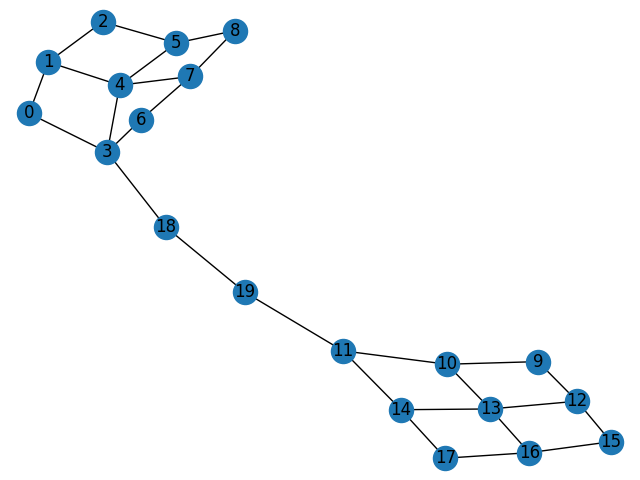
\includegraphics[width=0.7\textwidth]{environment.png}
\end{wrapfigure}

\begin{lstlisting}[label={lst:environment}]
ENVIRONMENT:
0: {0, 1, 3}
1: {0, 1, 2, 4}
2: {1, 2, 5}
3: {0, 3, 4, 6, 18}
4: {1, 3, 4, 5, 7}
5: {8, 2, 4, 5}
6: {3, 6, 7}
7: {8, 4, 6, 7}
8: {8, 5, 7}
9: {9, 10, 12}
10: {9, 10, 11, 13}
11: {19, 10, 11, 14}
12: {9, 12, 13, 15}
13: {10, 12, 13, 14, 16}
14: {17, 11, 13, 14}
15: {16, 12, 15}
16: {16, 17, 13, 15}
17: {16, 17, 14}
18: {19, 18, 3}
19: {11, 18, 19}
AGENTS:
[(14, 19), (17, 1)]
\end{lstlisting}


\section{SMT-based approach}\label{sec:smt-based-approach}
In the original paper the authors introduced a SAT-based approach while this implementation replaces it with a SMT-based one. 
Satisfiability Modulo Theories (SMT) solvers takes systems in arbitrary format (first-order logic), while SAT solvers are limited to Boolean equations and variables, nevertheless they still mantain the speed and automation of today's Boolean engines.
The authors of the paper developed their solution using the Picat language, we use the Z3 Solver's Python API: Z3Py.
The most difficult part is certainly represented by the constraint modeling and their adaptation for the Z3 Theorem Prover.
Following the original work, we define the following variables as Z3 Boolean Functions:

\begin{itemize}
\item $\forall x \in V, \forall a \in A, t \in {0, ..., T} : At(x, a, t)$ meaning that agent $a$ is at node $x$ at time step $t$.
\item $\forall(x, y)\in E, \forall a \in A, t \in {0, ..., T-1} : Pass(x, y, a, t)$ meaning that agent $a$ goes through arc $(x, y)$ at time step $t$. 
\end{itemize}

\begin{lstlisting}[label={lst:atpass}]
at_ = Function('at', IntSort(), IntSort(), IntSort(), BoolSort())
pass_ = Function('pass', IntSort(), IntSort(), IntSort(), IntSort(), BoolSort())
\end{lstlisting}

These variables are the problem unknowns and must be assigned to either true (1) or false (0).
We define as Z3 Integer Functions the following constant representations:

\begin{itemize}
\item $\forall a \in A : origin(a)$ which returns the initial position of the agent $a$.
\item $\forall a \in A : dest(a)$ which returns the goal position of the agent $a$.
\end{itemize}

\begin{lstlisting}[label={lst:origdest}]
orig_ = Function('orig', IntSort(), IntSort())
dest_ = Function('dest', IntSort(), IntSort())
\end{lstlisting}

The model is completed introducing the constraints on the variables:

% 1.1
\begin{description}\label{equation_set_1}
\item All agents must be in their initial position at time $t = 0$:
\begin{equation}
\forall a \in A: At(origin(a), a, 0) = 1
\label{eq:1.1}\end{equation}

% 1.2
\item All agents must be in their goal position at time $t = T$:
\begin{equation}
\forall a \in A : At(dest(a), a, T) = 1
\label{eq:1.2}\end{equation}

% 1.3
\item All agents can be in one node in every moment:
\begin{equation}
\forall a \in A, \forall t \in \{0,\dots,T\}: \displaystyle\sum_{x \in V}At(x,a,t)\leq1
\label{eq:1.3}\end{equation}

% 1.4
\item Every vertex must be occupied at most by an agent in every moment:
\begin{equation}\begin{split}
\forall x \in V, \forall t \in \{0,\dots,T\}: \displaystyle\sum_{a \in A}At(x,a,t)\leq1
\end{split}\label{eq:1.4}\end{equation}

% 1.5
\item If an agent is in a node it needs to leave by one of the outgoing arcs:
\begin{equation}\begin{split}
\forall x \in V, \forall a \in A, \forall t \in \{0,..,T-1\}: At(x,a,t) \\
\Rightarrow  \displaystyle\sum_{(x,y) \in E}Pass(x,y,a,t)=1
\end{split}\label{eq:1.5}\end{equation}

% 1.6
\item If an agent is using an arc, it must arrive at the corresponding node in the next time step
\begin{equation}\begin{split}
\forall (x,y) \in E, \forall a \in A, \forall t \in \{0,\dots,T-1\}: Pass(x,y,a,t) \\
\Rightarrow At(y,a,t+1)
\end{split}\label{eq:1.6}
\end{equation}

% 1.7
\item Two agents cannot exchange their positions:
\begin{equation}\begin{split}
\forall (x,y) \in E, x \neq y, \forall t \in \{0,\dots,T-1\}: \\
\displaystyle\sum_{a \in A}Pass(x,y,a,t) + Pass(y,x,a,t) \leq 1
\end{split}\label{eq:1.7}\end{equation}
\end{description}

The correct movements inside the graph are guided by the constraints~\ref{eq:1.5}-\ref{eq:1.7}, nevertheless it is not necessary to specify that each agent must make one and only on movement at a given instant $t$ because the spurious movements introduced by the constraint~\ref{eq:1.7} will never be performed thanks to~\ref{eq:1.5}.

The Z3 implementation is divided in three parts.
The details of the first one have been described before during variable and constant definitions. 
The second one defines intermediate variables useful to the definitions of the constraints in the third and last section.
In particular, the second part defines the summations present in the formal formulations of the original work, making easier to define the involved constraints.
For example the following code uses the Z3 function \textit{If} to map true variables to 1 and false variables to 0 cycling all combinations and summing over a certain ``dimension'' (for simplicity it is usually the inner one):

\begin{lstlisting}[label={lst:1.3.1}]
sum3_tmp = [[[If(at_(vertex, agent, time), 1, 0)
                       for vertex in range(edges_len)]
                      for time in range(makespan + 1)]
                     for agent in range(agents_len)]

sum3 = [[sum(sum3_tmp[agent][time])
         for time in range(makespan + 1)]
        for agent in range(agents_len)]

sum3 = [element for sublist in sum3 
            for element in sublist]
\end{lstlisting}

The resulting list is finally flatten and then used in the constraint~\ref{eq:1.3} in the following way:

\begin{lstlisting}[label={lst:1.3.2}]
s.add([vertex <= 1 for vertex in sum3])
\end{lstlisting}

The other constraints which do not use summations are solved using the Z3 function \textit{ForAll} like the~\ref{eq:1.6}

\begin{lstlisting}[label={lst:1.6}]
s.add([ForAll([x, y, a, t],
                  Implies(
                      And(x >= 0, x < edges_len, y >= 0, y < edges_len,
                          t >= 0, t <= makespan - 1, arc_(x, y),
                          pass_(x, y, a, t)),
                      at_(y, a, t + 1)
                  ))])
\end{lstlisting}

The variables \textit{x}, \textit{y}, \textit{a} and \textit{t} are Z3 Integer variables, which are bound independently to each \textit{ForAll} expression.
Because \textit{a} is used in the other \textit{ForAll} style constraints it has been similarly bound to a specific interval of integer values outside the shown piece of code.
\textit{arc\_} is a Boolean Z3 Function used to represent the presence of an arc between a couple of nodes.

To find an optimal makespan the makespan is increased until a satisfiable formula is generated.

\section{CP-based approach}\label{sec:cp-based-approach}

We now follow the paper showing how to formalize a MAPF problem as a scheduling problem.
Similarly to the authors we implement the model using the Python API of IBM ILOG CPLEX Studio: the library Docplex.
For this reason, the formal description uses some functions belonging to the grammar of the aforementioned IBM solver.
IBM ILOG CPLEX allows the definition of activities with interval variables.
The presence of an agent in a node can be seen as the activity of occupying that node for some amount of time and can be formulated in CPLEX as an interval variables that begins and finishes in a certain moment, represented by the predicates \textit{StartOf} and \textit{EndOf}.
The difference between the end time and the start time of the activity can be set using the predicate \textit{LengthOf}.
A great advantage of using interval variables is represented by their optionality, to check whether a certain activity is present or absent in the resulting schedule it is possible to use the predicate \textit{PresenceOf}.
In order to allow each agent to be able to visit the same node several times the authors developed a multi-layer model based on the copy of the original graph with some additional arcs that allow the transition between couples of graphs.
Let $l$ be the number of layers, namely the maximum number of times each agent can visit the same node.
In the original paper the layers belong to the set ${1,\dots,l}$, we decided to choose a zero-indexed approach such that our set of layers is ${0,\dots,l-1}$.
$\forall a \in A, \forall x \in V, \forall k \in {0,...,l-1}$ we considered the following optional activities:

\begin{itemize}
\item $N[x,a,k]$ corresponds to the time of an agent $a$ spent at node $x$ when the activity starts at layer $k$.
The start and end of this activity can span all over the available time, the length must be found.
\item $N^{in}[x,a,k]$ describes the time spent in the incoming arc at layer $k$.
\item $N^{out}[x,a,k]$ describes the time spent in the outgoing arc at layer $k$.
\item $A[x,y,a,k]$ where $k \in {0,...,l-1}$ which corresponds to transiting an agent $a$ from a node $x$ to the node $y$ at layer $k$.
The start and end of this activity can span all over the available time, the length is set to time required to traverse the arc.
\item $A[x,x,a,k]$ where $k \in {0,...,l-2}$ which corresponds to transiting an agent $a$ from a node $x$ to the node $x$ at layer $k$.
The start and end of this activity can span all over the available time, the length is set to zero because arcs between layers are not real.
\end{itemize}

We declare the described interval variables inside recursive Python data structures to easy access them using their parametric arguments as indexes.
For example \textit{N} is built using recursive lists representing in the following order the vertex, agent and layer dimensions, follows that the Pythonic \textit{N[x][a][k]} is equivalent to the formal $N[x,a,k]$.
On the other hand, we handle differently \textit{A}, because using a list of list is correct until the wanted operations are limited on cycling for each vertex its neighbors and access all of them using the index, which in this case is not the real identifier of the neighbor.
For example the nodes 5 and 6 are neighbors and \textit{A[4][0][a][k]} represents a movement between these two nodes, there is no way to refer the index 0 to the node 6, it could be for example another neighbor of 5, like the node 3.
In particular the constraint~\ref{eq:2.7} requires to use the neighbors of each node as origins for the \textit{A} interval variables.
To overcome this problem, we use a dictionary to explicitly access for an origin in \textit{A} (still represented as an index of the outermost list) its neighbors and their identifiers (keys of the dictionary).
Recalling the previous example \textit{A[4][6][a][k]} surely represents $A[5,6,a,k]$.
Probably substituting also the outer list with a dictionary would lead to a more clear model, but we decide to keep it for legacy with the other interval variables.
In order to simplify the implementation of some constraints we created two different interval variables to represent the following transitions $A[x,y,a,k]$ and $A[x,x,a,k]$.
Transitions from and to the same node are used by the solver to increase the layer (\ref{eq:2.11}) and to allow multiple visits to the same node by the same agent.
We represented these transitions defining the interval variables \textit{A\_equal}, which are indexed using only three values as the destination of the transition is always the origin itself and would be redundant.
Differently from \textit{A} interval variables which may have different lengths depending on the arc, \textit{A\_equal} variables have always length 0.

\begin{lstlisting}[label={lst:variables2}]
N = [[[interval_var(start=(0, upper_bound),
                    end=(0, upper_bound),
                    name="N_%s_%s_%s" % (vertex, agent, layer),
                    optional=True)
       for layer in range(num_layers)]
      for agent in range(agents_len)]
     for vertex in range(edges_len)]

A = [dict((neighbor, [[interval_var(start=(0, upper_bound),
                                    end=(0, upper_bound),
                                    length=1,
                                    name="A_%s_%s_%s_%s" %
                                     (vertex, neighbor, agent, layer),
                                    optional=True)
                       for layer in range(num_layers)]
                      for agent in range(agents_len)])
          for neighbor in edges[vertex] if vertex != neighbor)
     for vertex in range(edges_len)]


A_equal = [[[interval_var(start=(0, upper_bound),
                          end=(0, upper_bound),
                          length=0,
                          name="Ae_%s_%s_%s_%s" %
                           (vertex, vertex, agent, layer),
                          optional=True)
             for layer in range(num_layers - 1)]
            for agent in range(agents_len)]
           for vertex in range(edges_len)]
\end{lstlisting}

Also the variable indicating the final makespan must be declared
\begin{lstlisting}[label={lst:variablesmakespan}]
makespan = integer_var(0, upper_bound, name="MKSP")
\end{lstlisting}

We now introduce the constraints.
\begin{description}\label{eq:equation_set_2.1}
% 2.1
\item \begin{equation} PresenceOf(N[orig(a),a,0]) = 1 \label{eq:2.1}\end{equation}
% 2.2
\item \begin{equation} PresenceOf(N[dest(a),a,l-1]) = 1 \label{eq:2.2}\end{equation}
% 2.3
\item \begin{equation} PresenceOf(N^{in}[orig(a),a,0]) = 0 \label{eq:2.3}\end{equation}
% 2.4
\item \begin{equation} PresenceOf(N^{out}[dest(a),a,l-1]) = 0 \label{eq:2.4}\end{equation}
\end{description}

As already mentioned the formal representation is very similar to the implementation, for example the following constraints are almost identical to the formal definitions.

\begin{lstlisting}[label={lst:eq2.1-2.4}]
[model.add(presence_of(N[pair[0]][a][0]) == 1)
 for a, pair in enumerate(agents)]
[model.add(presence_of(N[pair[1]][a][num_layers - 1]) == 1)
 for a, pair in enumerate(agents)]
[model.add(presence_of(Nin[pair[0]][a][0]) == 0)
 for a, pair in enumerate(agents)]
[model.add(presence_of(Nout[pair[1]][a][num_layers - 1]) == 0)
 for a, pair in enumerate(agents)]
\end{lstlisting}

For this reason we decide to not comment all the constraints.

\begin{description}\label{eq:equation_set_2.2}
% 2.5
\item \begin{equation}\begin{split} \forall x \in V, \forall k \in \{0,\dots,l-1\}, x \neq orig(a) \lor k \neq 0: \\ PresenceOf(N[x,a,k]) \iff PresenceOf(N^{in}[x,a,k]) \end{split}\label{eq:2.5}\end{equation}
% 2.6
\item \begin{equation}\begin{split} \forall x \in V, \forall k \in \{0,\dots,l-1\}, x \neq dest(a) \lor k \neq l-1: \\ PresenceOf(N[x,a,k]) \iff PresenceOf(N^{out}[x,a,k]) \end{split}\label{eq:2.6}\end{equation}
% 2.7
\item \begin{equation}\begin{split} \forall x \in V, \forall k \in \{0,\dots,l-1\}: \\ Alternative(N^{in}[x,a,k], \{A[x,x,a,k-1]\} \cup \bigcup_{(y,x) \in E} A[y,x,a,k]) \end{split}\label{eq:2.7}\end{equation}
\end{description}

An interesting and already mentioned constraint is the~\ref{eq:2.7}.
Similarly to~\ref{eq:2.8} it defines the correct cardinality in which interval variables \textit{Nin}, \textit{A} and \textit{A\_equal} must be bound in the solution.
In particular, for each activity in the arcs incoming on a specific vertex, for an agent on a given layer there must be at most one traverse, possibly between different layers, if the layer is not the first, or from a neighbor occurring in the same layer.
To avoid indexes out of bound exceptions a control must be performed on the layer and a different constraint may be added to the model.

\begin{lstlisting}[label={lst:eq2.7}]
[model.add(
alternative(Nin[vertex][agent][layer],
            [A_equal[vertex][0][agent][layer - 1]] +
            [A[neighbor][vertex][agent][layer]
             for neighbor in edges[vertex].difference({vertex})]
            if layer > 0 else
            [A[neighbor][vertex][agent][layer]
             for neighbor in edges[vertex].difference({vertex})]
            ))
for layer in range(num_layers)
for agent in range(agents_len)
for vertex in range(edges_len)]
\end{lstlisting}

\begin{description}\label{eq:equation_set_2.3}
% 2.8
\item \begin{equation}\begin{split} \forall x \in V, \forall k \in \{0,\dots,l-1\}: \\ Alternative(N^{out}[x,a,k], \{A[x,x,a,k]\} \cup \bigcup_{(x,y) \in E} A[x,y,a,k]) \end{split}\label{eq:2.8}\end{equation}
% 2.9
\item \begin{equation}\begin{split} \forall (x,y) \in E, \forall k \in \{0,\dots,l-1\}: \\ PresenceOf(A[x,y,a,k]) \Rightarrow PresenceOf(N^{in}[y,a,k]) \end{split}\label{eq:2.9}\end{equation}
% 2.10
\item \begin{equation}\begin{split} \forall (x,y) \in E, \forall k \in \{0,\dots,l-1\}: \\ PresenceOf(A[x,y,a,k]) \Rightarrow PresenceOf(N^{out}[x,a,k]) \end{split}\label{eq:2.10}\end{equation}
% 2.11
\item \begin{equation}\begin{split} \forall x \in V, \forall k \in \{0,\dots,l-2\}: \\ PresenceOf(A[x,x,a,k]) \Rightarrow PresenceOf(N^{in}[x,a,k+1]) \end{split}\label{eq:2.11}\end{equation}
% 2.12
\item \begin{equation}\begin{split} \forall x \in V, \forall k \in \{0,\dots,l-2\}: \\ PresenceOf(A[x,x,a,k]) \Rightarrow PresenceOf(N^{out}[x,a,k]) \end{split}\label{eq:2.12}\end{equation}
% 2.13
\item \begin{equation} StartOf(N[orig(a),a,0]) = 0 \label{eq:2.13}\end{equation}
% 2.14
\item \begin{equation} EndOf(N[dest(a),a,l-1]) = MKSP \label{eq:2.14}\end{equation}
% 2.15
\item \begin{equation}\begin{split} \forall x \in V, \forall k \in \{0,\dots,l-1\}, x \neq orig(a) \lor k \neq 0: \\ StartOf(N[x,a,k]) = EndOf(N^{in}[x,a,k]) \end{split}\label{eq:2.15}\end{equation}
% 2.16
\item \begin{equation}\begin{split} \forall x \in V, \forall k \in \{0,\dots,l-1\}, x \neq dest(a) \lor k \neq l-1: \\ EndOf(N[x,a,k]) = StartOf(N^{out}[x,a,k]) \end{split}\label{eq:2.16}\end{equation}
% 2.17
\item \begin{equation}\begin{split} \forall x \in V: \\ NoOverlap(\bigcup_{a \in A, k \in \{1,\dots,l-1\}} N[x,a,k])\end{split}\label{eq:2.17}\end{equation}
\end{description}

The constraint~\ref{eq:2.17} represents another interesting case.
The \textit{no\_overlap} function constrains a set of interval variables not to overlap each others.
By default (like in the~\ref{eq:2.18} implementation) it can receive a list of interval variables and it will constraint them to not overlap and to be at least distant one to another (the difference between the start of one and end of another, where the former succeeds the latter) zero.
In order to modify this behavior we pass a \textit{sequence\_var} containing the interval variables and we create a transition matrix which represents for each combination of variables the minimum distance they must maintain.

\begin{lstlisting}[label={lst:minimize2}]
tm_size = num_layers * agents_len
tm = transition_matrix(tm_size)

for i in range(tm_size):
    for j in range(tm_size):
        if j not in range((i // num_layers) * num_layers, (i // num_layers) * num_layers + num_layers):
            tm.set_value(i, j, 1)

[model.add(no_overlap(sequence_var([N[vertex][agent][layer]
                                    for agent in range(agents_len)
                                    for layer in range(num_layers)]), tm))
 for vertex in range(edges_len)]
\end{lstlisting}

For a specific vertex (notice the outer loop on vertices) the same agent can occupy the same node in different layers with a distance between each possible pair at minimum 0, because traversing layers is not a real movement and occurs immediately.
On the other hand, between different agents in the same or different layers, the distance between possible pairs must be at least 1.

\begin{description}\label{eq:equation_set_2.4}
% 2.18
\item \begin{equation}\begin{split} \forall (x, y) \in E: \\ NoOverlap(\bigcup_{a \in A, k \in \{1,\dots,l-1\}} \{A[x,y,a,k], A[y,x,a,k]\})\end{split}\label{eq:2.18}\end{equation}
\end{description}

Finally a minimization constraint is added for the makespan variable.
\begin{lstlisting}[label={lst:minimize2}]
model.add(model.minimize(makespan))
\end{lstlisting}

\section{Results}\label{sec:results}
This section is dedicated to the description and analysis of the results we obtained from the tests.
The aim is to compare the two approaches that we have previously described to solve the MAPF problem,
in particular, we used the following performance parameters:

\begin{description}
    \item $solving_time$: measured in seconds.
    \item $memory_{usage}$: memory occupied in MB.
    \item $n_{conflicts}$: number of conflicts.
    \item $n_{decision}$: number of decision points.
\end{description}

Let's recall that for the SMT-based approach we used Z3 while we used IBM CP Optimizer
for the scheduling approach. The latter provides the possibility to perform a parallel search,
in this regard we have used 8 workers (default value).
\subsection{Implementation}\label{subsec:implementation}
We used the Python package NetworkX for the creation, manipulation of complex networks.
This framework provides also many standard graph algorithms, like finding an agent's shortest path,
which was used in the scheduling-based approach to compute the optimal number of layers. For this purpose
we have implemented the solving MAPF algorithm described by R. Barták, J. Švancara and M. Vlk with a little variation:
we used a heuristic upper bound rather than computing it with $PaS$ algorithm and we also
used it as upper bound of $num_{layers}$ in the search cycle of the first feasible solution. This is
beacause $PaS$, in addition to compute the upper bound, performs a first check on the existence of a feasible solution
to the problem. Since we started from a heuristic upper bound, we moved the control of the existence of a solution
introducing, in fact, an upper bound also for the $num_{layers}$. Instead regarding the SAT-based approach,
we used a cycle starting with $makespan = 0$ and increasing it until a feasible solution is found. In this way we are
sure that the first feasible solution found is also the best. Therefore the tests we carried out are baed on the comparison
of the performance of these two approaches, according to the parameters described above, in the execution
with the optimal $num_{layers}$ for the SMT-based approach, and with the maekespan which returns the first
feasible solution, for the SAT-based approach. Finally, a test can be briefly described like this:
\begin{enumerate}
    \item Graph generation with NetworkX
    \item Choice of the number of agents according to a certain criterion (for example proportional to the number of nodes in the graph) and random choice of the departure and arrival node for each
    \item Execution of the resolution algorithms for both approaches described above
    \item Storage of performance parameters of the two algorithms executed with the optimal parameters
    \item Increase in the size of the graph up to a predetermined $MAX_{SIZE}$ (in some tests)
    \item Plot of the results
\end{enumerate}
From an implementation point of view we have developed an interface that would allow us to perform various tests in a flexible way.
\subsection{Testing}\label{subsec:testing}
The first test was performed on a two-dimensional grid generated by NetworkX by varying the size from $MIN_SIZE=2$ to $MAX_SIZE=6$.
Also the number of agents varies with the size of the graph, in particular following the relationship $n_agents = SIZE_i$ where $SIZE_i$ is the size of the graph in step $i$.
This is to evaluate the performance of the two approaches to increasing the the complexity of the problem which, in general, is proportional to the size of the graph and the number of agents.
\end{document}
